\begin{figure}[t]\centering
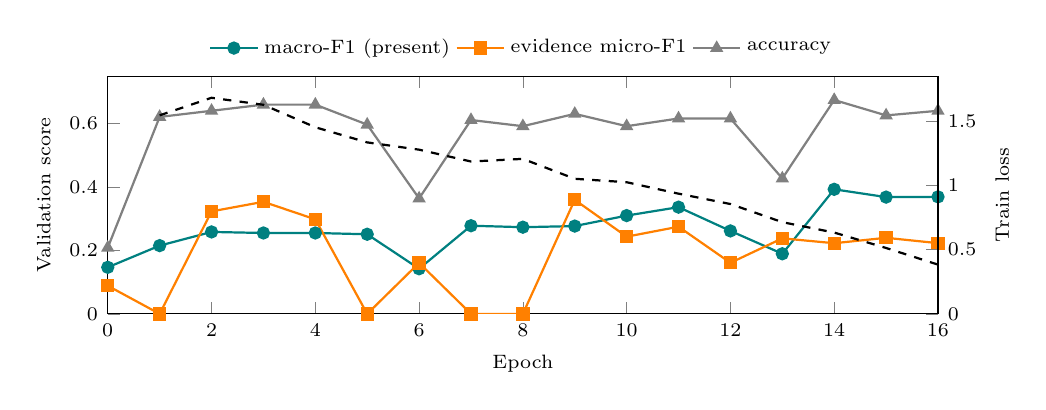
\begin{tikzpicture}\begin{axis}[width=\columnwidth,height=4.6cm,xlabel={Epoch},ylabel={Validation score},ymin=0,ymax=0.75,
legend style={font=\scriptsize,at={(0.5,1.03)},anchor=south,legend columns=3,draw=none},tick label style={font=\scriptsize},label style={font=\scriptsize},
axis y line*=left,xmin=0,xmax=16]
\addplot[thick,mark=*,color=teal] coordinates {(0,0.1469) (1,0.2153) (2,0.2585) (3,0.2552) (4,0.2552) (5,0.2512) (6,0.1423) (7,0.2781) (8,0.2735) (9,0.2770) (10,0.3101) (11,0.3367) (12,0.2617) (13,0.1896) (14,0.3930) (15,0.3684) (16,0.3692)};\addlegendentry{macro-F1 (present)}
\addplot[thick,mark=square*,color=orange] coordinates {(0,0.0887) (1,0.0000) (2,0.3234) (3,0.3536) (4,0.2983) (5,0.0000) (6,0.1609) (7,0.0000) (8,0.0000) (9,0.3598) (10,0.2436) (11,0.2750) (12,0.1611) (13,0.2383) (14,0.2229) (15,0.2400) (16,0.2231)};\addlegendentry{evidence micro-F1}
\addplot[thick,mark=triangle*,color=gray] coordinates {(0,0.2087) (1,0.6214) (2,0.6408) (3,0.6602) (4,0.6602) (5,0.5971) (6,0.3641) (7,0.6117) (8,0.5922) (9,0.6311) (10,0.5922) (11,0.6165) (12,0.6165) (13,0.4272) (14,0.6748) (15,0.6262) (16,0.6408)};\addlegendentry{accuracy}
\end{axis}
\begin{axis}[width=\columnwidth,height=4.6cm,axis y line*=right,axis x line=none,ylabel={Train loss},ymin=0,xmin=0,xmax=16,
tick label style={font=\scriptsize},label style={font=\scriptsize}]
\addplot[dashed,thick,color=black] coordinates {(1,1.5429) (2,1.6790) (3,1.6247) (4,1.4500) (5,1.3324) (6,1.2759) (7,1.1839) (8,1.2044) (9,1.0496) (10,1.0229) (11,0.9339) (12,0.8535) (13,0.7125) (14,0.6317) (15,0.5119) (16,0.3827)};
\end{axis}\end{tikzpicture}
\caption{Validation metrics per epoch (solid, left axis; epoch 0 is the unadapted base) and mean training loss (dashed, right axis). The checkpoint with the best selection score (epoch 9) was frozen.}\label{fig:train}\end{figure}

\begin{figure}[t]\centering
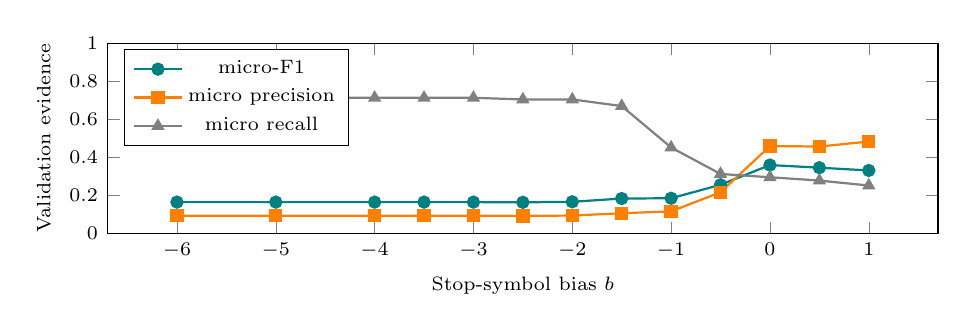
\begin{tikzpicture}\begin{axis}[width=\columnwidth,height=4cm,xlabel={Stop-symbol bias $b$},ylabel={Validation evidence},ymin=0,ymax=1,
legend style={font=\scriptsize,at={(0.02,0.97)},anchor=north west},tick label style={font=\scriptsize},label style={font=\scriptsize}]
\addplot[thick,mark=*,color=teal] coordinates {(1,0.3314) (0.5,0.3459) (0,0.3598) (-0.5,0.2562) (-1,0.1854) (-1.5,0.1840) (-2,0.1668) (-2.5,0.1641) (-3,0.1652) (-3.5,0.1652) (-4,0.1652) (-5,0.1652) (-6,0.1652)};\addlegendentry{micro-F1}
\addplot[thick,mark=square*,color=orange] coordinates {(1,0.4833) (0.5,0.4571) (0,0.4595) (-0.5,0.2169) (-1,0.1166) (-1.5,0.1066) (-2,0.0946) (-2.5,0.0929) (-3,0.0934) (-3.5,0.0934) (-4,0.0934) (-5,0.0934) (-6,0.0934)};\addlegendentry{micro precision}
\addplot[thick,mark=triangle*,color=gray] coordinates {(1,0.2522) (0.5,0.2783) (0,0.2957) (-0.5,0.3130) (-1,0.4522) (-1.5,0.6696) (-2,0.7043) (-2.5,0.7043) (-3,0.7130) (-3.5,0.7130) (-4,0.7130) (-5,0.7130) (-6,0.7130)};\addlegendentry{micro recall}
\end{axis}\end{tikzpicture}
\caption{Validation-only sweep of the additive stop-symbol bias. Lower $b$ makes the decoder cite more sentences, trading precision for recall; $b=0$ maximises micro-F1 and was frozen before testing.}\label{fig:cal}\end{figure}
